\chapter{Metodologia}
\label{ch:4metodologia}

\section{Classificação da pesquisa}

Este trabalho adota uma abordagem metodológica \textbf{mista}, combinando uma revisão sistemática da literatura com uma análise experimental controlada. Trata-se de um estudo de natureza \textbf{aplicada}, no qual diferentes protocolos de comunicação entre microsserviços são avaliados empiricamente. Os objetivos do estudo demandam a medição objetiva de desempenho (latência, vazão, uso de recursos, etc.) sob cada protocolo, o que justifica a escolha por um delineamento experimental. Alternativas como análises puramente teóricas ou simulações não seriam adequadas para capturar todas as nuances de desempenho em um ambiente real. Por isso, optou-se por implementar um cenário de teste concreto e coletar métricas diretamente, permitindo a quantificação das diferenças de performance e uso de recursos além da verificação da superioridade de algum protocolo em termos práticos. Além disso, por meio de comparações estatísticas, busca-se verificar se eventuais diferenças observadas são estatisticamente significativas e relevantes.

No contexto deste trabalho, realizou-se uma série de testes de uso em uma aplicação distribuída em microsserviços de um protótipo de assistente virtual multimodal com \acrfull{ia} generativa, utilizando exemplos do setor financeiro como cenários. Em suma, a metodologia foi planejada para garantir validade interna, controlando variáveis relevantes, produzindo dados quantitativos confiáveis e possibilitando a comparação direta entre as três abordagens de comunicação.

\section{Etapas da pesquisa}
Esta pesquisa pode ser divida em 4 etapas:

\begin{itemize}
    \item \textbf{Revisão bibliográfica}: Esta etapa consistiu em um estudo aprofundado das principais tecnologias de microsserviços e orquestração, detalhada no \autoref{ch:2pilares} e no \autoref{ch:3estado_da_arte}. O objetivo foi estabelecer uma base teórica sólida e, ao mesmo tempo, buscar por análises comparativas similares, garantindo a originalidade e a relevância da pesquisa.
    
    \item \textbf{Desenvolvimento da arquitetura de testes}: Nesta fase, descrita na \autoref{sec:4-arquitetura_testes}, o objetivo foi projetar e implementar a arquitetura de microsserviços do assistente virtual. Isso incluiu o desenvolvimento dos serviços individuais (\acrshort{stt}, \acrshort{llm}, \acrshort{tts}), a definição das interfaces de comunicação e a configuração de um ambiente de teste controlado para garantir a fidelidade do experimento.
    
    \item \textbf{Experimentos}: Esta etapa foi a execução prática dos testes, detalhada na \autoref{sec:4-procedimentos_experimentais}. Nela, o sistema foi submetido a diferentes cenários de demanda (simples, tradicional e complexa) para coletar dados quantitativos sobre o comportamento de cada protocolo de comunicação sob variadas condições de estresse.
    
    \item \textbf{Análise de dados}: O objetivo final foi processar e interpretar os dados brutos coletados durante os experimentos, conforme apresentado no \autoref{ch:5resultados}. As métricas de desempenho e uso de recursos foram analisadas para extrair \textit{insights} significativos, identificar padrões e, finalmente, formular as conclusões do estudo.
\end{itemize}



\section{Arquitetura de testes}
\label{sec:4-arquitetura_testes}

O experimento foi elaborado com base em uma arquitetura de microsserviços representativa de um assistente virtual multimodal com \acrfull{ia} generativa. A \autoref{fig:4-arquitetura-experimentos} ilustra a arquitetura proposta, a qual consiste em um serviço orquestrador (\textit{gateway} do assistente) que recebe as requisições dos usuários e coordena chamadas para serviços especializados de \textit{backend}. Cada teste isolou um protocolo de comunicação de cada vez (\gls{rest}, \gls{grpc} ou Thrift) para permitir uma comparação justa dos resultados. Esse delineamento possibilitou identificar o impacto do mecanismo de orquestração na performance do sistema, alinhando-se aos objetivos de determinar qual tecnologia oferece menor latência e maior eficiência. 

\begin{figure}[H]
\caption{Arquitetura de microsserviços do assistente virtual multimodal}
\label{fig:4-arquitetura-experimentos}
\centering
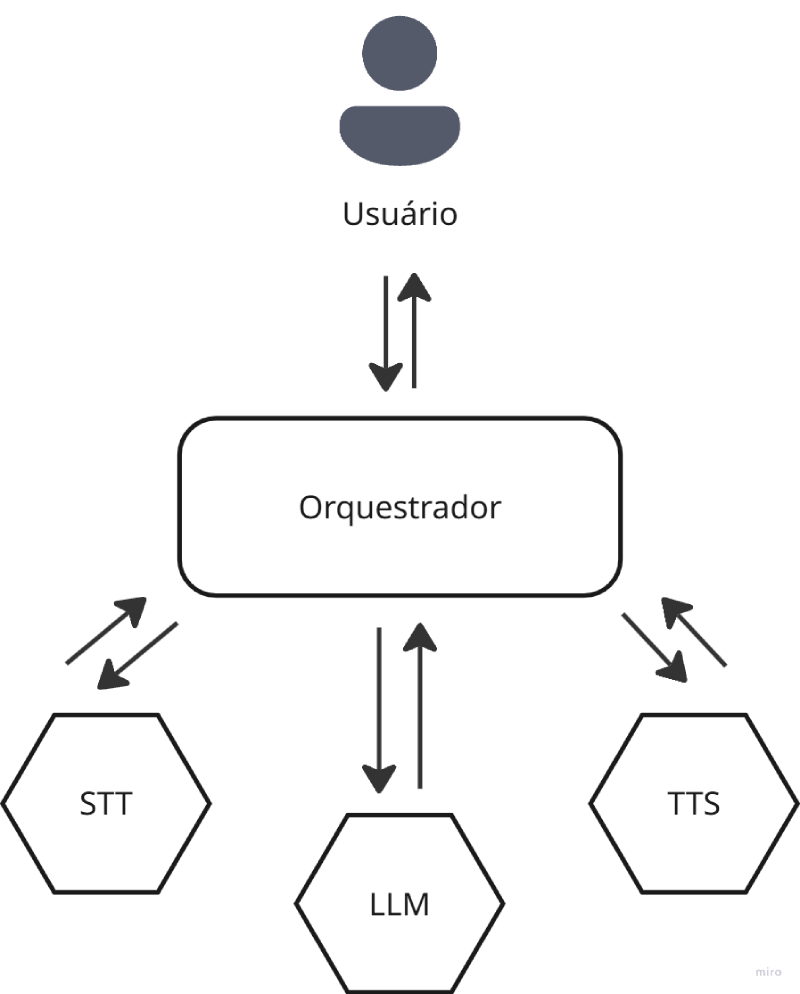
\includegraphics[width=0.4\textwidth]{imagens/4-arquitetura_cenario.png}
{\par \raggedright \footnotesize Fonte: Elaborado pelo autor.}
\end{figure}

Com arquivos de áudios pré-definidos, simularam-se cenários de interação por voz (Detalhado em \ref{sec:4-procedimentos_experimentais}), onde o orquestrador aciona um microserviço de reconhecimento de fala (\acrshort{stt}) que converte áudio em texto e, em seguida, encaminha esse texto ao serviço de \gls{ia} generativa (\acrshort{llm}). A resposta textual pode ser, posteriormente, enviada a um microserviço de síntese de voz (\acrshort{tts}) que retorna áudio ao usuário. Todos esses serviços (\acrshort{stt}, \acrshort{llm}, \acrshort{tts}) são implementados como microsserviços independentes que se comunicam por meio de rede. Essa divisão reflete cenários reais de assistentes multimodais, nos quais diferentes módulos gerenciam modalidades distintas de dados (texto, voz e imagem) em um fluxo de processamento.

Para fins do experimento, a arquitetura acima foi implantada em três configurações distintas, variando apenas o protocolo de comunicação utilizado nas chamadas remotas:

\begin{itemize}
\item \textbf{Configuração \gls{rest}}: todos os microsserviços expõem \gls{api}s \gls{rest} (\acrshort{http}/1.1 com \acrshort{json}). O serviço orquestrador invoca os demais via chamadas \acrshort{http} \gls{rest} tradicionais (endpoints RESTful).
\item \textbf{Configuração \gls{grpc}}: os microsserviços utilizam \gls{grpc} sobre \acrshort{http}/2, com interfaces definidas em arquivos \texttt{.proto} e dados serializados em \textit{Protocolo Buffers}. O orquestrador atua como cliente \gls{grpc} para os outros serviços, usando esquemas gerados a partir dos \texttt{.proto}.
\item \textbf{Configuração Thrift}: os microsserviços comunicam-se via Apache Thrift, utilizando uma interface Thrift comum. O orquestrador chama os serviços através dos clientes Thrift gerados.
\end{itemize}

Em cada configuração, a lógica de negócio dos microsserviços permanece idêntica, assim como os dados trocados e a sequência de chamadas no pipeline do assistente. Dessa forma, isola-se o impacto do protocolo de comunicação, garantindo que quaisquer diferenças de desempenho sejam atribuídas, principalmente, ao \textit{overhead} de comunicação (formato de serialização, transporte etc.) e não à funcionalidade em si. Cada protocolo foi avaliado separadamente, iniciando o experimento com \gls{rest}, seguido pela repetição com \gls{grpc} e, por fim, com Thrift.

É importante ressaltar que, para possibilitar a troca do protocolo de forma transparente, foram desenvolvidas adaptações ou interfaces duplas quando necessário. Definiram-se modelos de dados equivalentes em \acrshort{json}, mensagens \textit{Protocol} Buffers e \textit{structs} Thrift, assegurando a mesma uniformidade de conteúdo e o tamanho do \textit{payload} em cada cenário. Isso garantiu a comparabilidade direta. Durante cada execução, apenas um protocolo permaneceu ativo, prevenindo interferências mútuas. Assim, obtêm-se medidas repetidas para cada protocolo, permitindo análises emparelhadas e redução de variabilidade.

\subsubsection{Justificativa da Seleção de Protocolos}
\label{subsec:justificativa-protocolos}

A seleção dos protocolos \acrshort{rest}, \acrshort{grpc} e Apache Thrift para esta pesquisa foi fundamentada em critérios que buscam abranger os paradigmas de comunicação mais relevantes e adotados na indústria para orquestração de microsserviços, conforme comparado anteriomente na \autoref{tab:2-protocolos}.

O protocolo \acrshort{rest} foi incluído por representar o padrão \textit{de facto} e amplamente consolidado para APIs web. Sua ubiquidade, simplicidade de implementação e interoperabilidade o tornam uma base obrigatória para qualquer análise comparativa, servindo como \textit{baseline} para mensurar ganhos de performance de alternativas mais modernas.

Os protocolos \acrshort{grpc} e Apache Thrift foram selecionados por representarem o estado da arte em comunicação binária eficiente. Ambos utilizam serialização binária (\textit{Protocol Buffers} e formato binário próprio, respectivamente) e operam sobre protocolos de transporte modernos (\acrshort{http}/2 e \acrshort{tcp}), sendo projetados especificamente para oferecer alta performance e baixa latência em ambientes de sistemas distribuídos. Sua inclusão permite avaliar o trade-off entre a simplicidade do \acrshort{rest} e a eficiência de soluções orientadas a performance.

Optou-se por não incluir tecnologias como \acrshort{graphql} ou Apache Kafka no escopo experimental deste estudo. Ambas as soluções, embora relevantes em contextos específicos, introduziriam variáveis arquiteturais que comprometeriam a equivalência direta desejada para esta análise comparativa. O \acrshort{graphql} normalmente requer um gateway ou camada de agregação, introduzindo um componente intermediário não presente na comunicação ponto a ponto avaliada nos demais protocolos. O Kafka atua primordialmente em paradigmas assíncronos de mensageria, enquanto o foco desta pesquisa reside estritamente na comunicação síncrona entre microsserviços em um pipeline de IA multimodal, cujos contratos são fixos e conhecidos. Essa escolha por protocolos de comunicação direta e síncrona possibilitou a manutenção da equivalência arquitetural entre os cenários testados, isolando o impacto do protocolo de comunicação como variável principal.

Portanto, a tríade \acrshort{rest}-\acrshort{grpc}-Thrift forma um conjunto representativo e tecnicamente contrastante, permitindo uma análise abrangente entre o padrão textual ubíquo (\acrshort{rest}) e as principais alternativas binárias de alto desempenho (\acrshort{grpc} e Thrift).

\subsection{Ambiente de Teste}

Os experimentos ocorreram em um ambiente de teste controlado, configurado em uma nuvem privada, com o intuito de replicar condições realistas de produção e isolar fatores externos, como flutuações na rede, processos agendados do sistema operacional e interferência de outras aplicações. Dessa forma, toda a infraestrutura foi configurada utilizando \textbf{contêineres Docker}, o que representa um ambiente típico de microsserviços em escala. Essa escolha possibilita a reprodução do experimento e assegura que cada modelo seja executado em um contêiner isolado, com controle sobre alocações de CPU e memória, evitando interferências.

Em termos de hardware, utilizou-se um servidor dedicado com  capacidade suficiente para executar modelos de \gls{ia} que integram os microsserviços, como \acrshort{stt}, \acrshort{llm} e \acrshort{tts}, conforme detalhado na \autoref{tab:4-especificacoes-hardware}. 

\begin{table}[H]
\centering
\caption{Especificações do hardware utilizado nos experimentos}
\label{tab:4-especificacoes-hardware}
\begin{tabularx}{\linewidth}{|l|X|}
\hline
\textbf{Componente} & \textbf{Especificação} \\
\hline
Processadores (CPU) & Processador Intel Xeon Platinum 8273CL @ 2.20GHz (turbo 2.9 GHz); 12 núcleos/24 threads por soquete; \\
\hline
Memória \acrshort{ram} & 85GB disponíveis; \textit{sem swap}. \\
\hline
Armazenamento & Sistema: 200GB; Dados: NVMe 2TB. \\
\hline
Placa Gráfica (\acrshort{gpu}) & NVIDIA Tesla A100 de 40 GB \\
\hline
Sistema Operacional & Oracle Linux Server 9.6 (\texttt{platform:el9}); arquitetura x86\_64 \\
\hline
Referência GCP & a2-highgpu-1g \\
\hline
\end{tabularx}
{\par \raggedright \footnotesize Fonte: Elaborado pelo autor.\par}
\end{table}

\subsubsection{Justificativa do Ambiente de Alto Desempenho}
\label{subsec:justificativa-hardware}

Os experimentos foram conduzidos em um ambiente de alto desempenho, conforme detalhado na \autoref{tab:4-especificacoes-hardware}. Esta escolha foi intencional e estrategicamente alinhada ao objetivo central do estudo: isolar e avaliar o impacto dos protocolos de comunicação na orquestração de microsserviços, minimizando interferências relacionadas a limitações de hardware no processamento de modelos de IA.

Em testes preliminares realizados em ambientes com recursos computacionais modestos, observou-se que a carga inerente ao processamento de modelos de IA generativa, especialmente modelos grandes como Whisper e LLMs, consumia a maior parte dos recursos de CPU e , configurando-se como um gargalo dominante. Nessas condições, as diferenças de desempenho entre os protocolos de comunicação tornaram-se marginalmente perceptíveis, uma vez que a latência foi majoritariamente determinada pelo tempo de inferência dos modelos e não pela eficiência da comunicação entre os serviços.

Ao utilizar um hardware compatível, assegurou-se que os modelos de IA operassem dentro de patamares de latência previsíveis, além de garantir recursos suficientes para lidar com a carga de processamento multimodal. Dessa forma, o impacto relativo da comunicação entre microsserviços pôde ser amplificado e observado de maneira mais clara e isolada, atendendo ao propósito comparativo do estudo.

O foco nesta fase foi avaliar o comportamento dos protocolos em condições ideais de processamento, estabelecendo um \textit{baseline} de desempenho livre de ruídos causados pela escassez de recursos. Estudos futuros poderão investigar o comportamento desses protocolos em ambientes com restrições de hardware ou em arquiteturas híbridas, expandindo a aplicabilidade das conclusões.

\section{Procedimentos Experimentais}
\label{sec:4-procedimentos_experimentais}

Nesta seção são descritos os procedimentos experimentais em detalhe, incluindo o planejamento das execuções, geração de cenário e coleta de dados. O experimento seguiu um protocolo padronizado para cada configuração de teste (\gls{rest}, \gls{grpc}, Thrift), variando apenas o protocolo em uso.

\subsection{\textit{Workloads} e Cenários de Teste}

Todos os cenários de demanda definidos para este experimento simulam interações via \textbf{entrada de voz}, variando apenas o nível de complexidade cognitiva da solicitação feita ao assistente virtual. Em cada caso, a entrada de voz é processada pelo pipeline completo de microsserviços: \acrfull{stt}, processamento de linguagem natural e raciocínio por \acrfull{llm}, e, por fim,  \acrfull{tts} para entrega da resposta.

Foram definidos três cenários:

\begin{itemize}
    \item \textbf{Cenário 1 (simples)}: Solicitação objetiva e direta, que requer apenas uma busca simples de informação factual. Para este cenário, não injetamos nenhum contexto extra. \\
    Áudio: "Qual é o código do ativo da Petrobras?" \\
    Esse cenário envolve processamento mínimo no \gls{llm}, com baixa demanda de inferência e retorno rápido.
    \item \textbf{Cenário 2 (tradicional)}: Pergunta de dificuldade intermediária, que exige interpretação conceitual e comparação entre dois elementos do domínio financeiro. Para este cenário, injetamos o contexto de um manual do investidor, como o disponibilizado pela CVM\footnote{Disponível em: \url{https://www.gov.br/investidor/pt-br/educacional/programa-bem-estar-financeiro/programa-bem-estar-financeiro-arquivos/apostila-06.pdf}. Acesso em: 26 jul. 2025.}. \\
    Áudio: "Qual a diferença entre renda fixa e Ibovespa?" \\
    Esse cenário requer raciocínio moderado no \gls{llm}, incluindo compreensão de conceitos e elaboração de resposta explicativa.
    \item \textbf{Cenário 3 (complexo)}: Consulta complexa que demanda análise de dados históricos e síntese de informações. Para este cenário, fornecemos um contexto com dados diários das ações de 2024 em formato \gls{csv}, simulando a consulta a uma fonte interna de informações de mercado. \\
    Áudio: "Quais foram as melhores ações de 2024?" \\
    Esse cenário impõe maior tempo de raciocínio ao \gls{llm}, podendo envolver consultas a fontes internas, ordenação e seleção de dados para compor a resposta.
\end{itemize}

A justificativa para os cenários propostos está em simular o comportamento de um aplicativo de informações e análise para investidores, um público-alvo que hoje representa 59 milhões de investidores individuais na B3 \cite{anbima_raio_nodate}. A diversidade de usuários e a natureza de suas interações diárias foram a base para a concepção dos três níveis de demanda. O Cenário Simples reflete o comportamento de investidores iniciantes, que buscam informações simples para aprender sobre o mercado. O Cenário Tradicional representa o investidor tradicional, com dúvidas cotidianas e a necessidade de comparar conceitos e ativos. Já o Cenário Complexo simula o usuário mais experiente, que busca extrair informações úteis e realizar análises aprofundadas para tomar decisões de investimento, impondo uma carga de processamento significativamente maior ao sistema. Deste modo, os cenários foram desenhados para representar o comportamento agregado de uma carteira de clientes, e não de um único usuário, validando a abordagem em um contexto de aplicação real e em escala.

Em todos os cenários, o fluxo de processamento é idêntico: o áudio da pergunta é enviado ao serviço de \gls{stt}, convertido em texto, processado pelo \gls{llm} para gerar a resposta textual e, finalmente, sintetizado em áudio pelo serviço de \gls{tts}. A variação no tempo de resposta e no consumo de recursos ocorre principalmente em função da complexidade do raciocínio exigido em cada cenário, permitindo avaliar o impacto do protocolo de comunicação em diferentes níveis de carga cognitiva.

\subsection{Execução dos Testes}

Para a execução dos cenários de testes, utilizou-se uma combinação de duas ferramentas: k6\footnote{Disponível em \url{https://k6.io}} para a geração de carga e coleta de métricas do lado do cliente, e Prometheus\footnote{Disponível em \url{https://prometheus.io}} para o monitoramento de recursos do lado do servidor. Com o k6, foram desenvolvidos scripts em JavaScript para simular o comportamento dos usuários em cada um dos cenários definidos (simples, tradicional e complexo). Esses scripts foram configurados para realizar chamadas ao endpoint do serviço orquestrador, enviando os áudios pré-definidos e medindo as métricas de resultado, como latência (p50, p95, p99), throughput e taxas de erro. Em paralelo, o ambiente foi instrumentado com o Prometheus para coletar, em tempo real, as métricas de desempenho da infraestrutura. Por meio de exporters configurados nos contêineres, o Prometheus monitorou o uso de CPU e memória de cada microsserviço, fornecendo uma visão detalhada do consumo de recursos sob estresse.

Cada configuração de protocolo (\gls{rest}, \gls{grpc} e Thrift) foi submetida ao mesmo rigor de testes, com 15 replicações independentes por protocolo para garantir um tamanho amostral estatisticamente relevante. Entre a avaliação de cada protocolo, o sistema era reiniciado para limpar completamente o estado e evitar interferências entre os testes. A ordem de execução dos cenários foi randomizada para todos os protocolos, o que evitou viés e assegurou que a única variável entre os experimentos fosse a tecnologia de comunicação, permitindo uma comparação direta e justa dos resultados.

Durante todos os experimentos, o ambiente foi monitorado para identificar anomalias ou interferências externas, como picos de CPU na máquina host ou atividades de rede não relacionadas ao teste, garantindo que nenhuma condição externa contaminasse os resultados. Não foi necessário descartar nenhuma execução por comportamento anômalo. Ao final dos procedimentos, obteve-se um conjunto robusto de dados brutos, incluindo tempos de resposta de milhares de requisições e a utilização de recursos por microsserviço, que foram agregados e analisados nas seções subsequentes.

\section{Métricas e Variáveis de Avaliação}
\label{sec:5-metricas-variaveis}

Foram definidas algumas \textbf{métricas de desempenho} para avaliar quantitativamente cada protocolo. As métricas escolhidas contemplam aspectos de latência de resposta (incluindo cauda), capacidade de throughput, eficiência de recursos e confiabilidade. A \textbf{\autoref{tab:4-metricas}} resume as principais métricas coletadas e suas definições.

\begin{table}[H]
\centering
\caption{Métricas coletadas nos experimentos e sua descrição.}
\label{tab:4-metricas}
\begin{tabularx}{\linewidth}{|p{4cm}|X|}
\hline
\textbf{Métrica} & \textbf{Descrição} \\
\hline
\textit{Latência (p50, p95, p99)} & Tempo de resposta end-to-end, em milissegundos (ms), desde a chegada da requisição ao orquestrador até o envio completo da resposta ao cliente. Reporta-se a mediana (p50) e as latências de cauda (p95 e p99), fundamentais em contextos financeiros por evidenciarem picos que podem impactar a experiência do usuário e operações sensíveis. \\
\hline
\textit{Vazão} (Throughput) & Número de requisições processadas por segundo pelo sistema. Mede a capacidade de atendimento sob carga, normalmente expresso em req/s. \\
\hline
\textit{Uso de CPU} & Porcentagem de utilização do(s) CPU(s) pelos microsserviços durante o teste. Medido como média de CPU time total consumido. Indica a eficiência computacional do protocolo. \\
\hline
\textit{Uso de Memória} & Quantidade de memória \acrshort{ram} ocupada pelos serviços durante a execução. Ajuda a identificar \textit{overhead} de alocação de memória de cada framework. \\
\hline
\textit{Taxa de Erro} & Porcentagem de requisições que resultaram em erro (código \acrshort{http} \$\ge\$ 400 ou exceções nas chamadas \gls{rpc}) ou \textit{timeout}. Mede a confiabilidade sob estresse. Espera-se taxas de erro baixas (idealmente 0\%). \\
\hline
\end{tabularx}
{\par \raggedright \footnotesize Fonte: Elaborado pelo autor.\par}
\end{table}

Essas métricas foram escolhidas para cobrir tanto a perspectiva do usuário final (latência, taxa de erro) que afetam diretamente a qualidade do serviço percebida, quanto a perspectiva do provedor do serviço (throughput, uso de CPU/memória) que afetam escalabilidade e custo. Em alinhamento com trabalhos correlatos e diretrizes de avaliação de \gls{api}s, focou-se especialmente em \textbf{tempos de resposta e throughput}, bem como em métricas de \textbf{uso de recursos}. Em particular, a análise de \textbf{latência de cauda (p95 e p99)} fornece uma visão mais realista do comportamento sob pico do que medidas de tendência central isoladas.

A latência medida \textit{end-to-end} foi computada para cada requisição individual. Os percentis \textit{p50}, \textit{p95} e \textit{p99} foram calculados a partir do conjunto dessas observações por cenário e replicação. O \textit{throughput} foi inferido tanto pelo lado do cliente (número total de requisições concluídas dividido pelo tempo de teste) quanto monitorado no lado servidor (contadores de requisições por segundo). As métricas de \textit{uso de CPU e memória} foram coletadas via Prometheus a cada intervalo de 5 segundos durante os testes. A \textit{taxa de erro} foi medida pelo gerador de carga: qualquer resposta inválida ou ausência de resposta dentro de um tempo limite de 6 segundos (\textit{timeout}) foi contabilizada como erro.

Todas as métricas foram registradas para cada replicação de teste, permitindo agregações simples e comparações diretas entre protocolos. Para latência, reportam-se explicitamente \textit{p50}, \textit{p95} e \textit{p99}; quando necessário para sumarização entre replicações, utiliza-se a média desses percentis por cenário.

\subsection{Variáveis, fatores e métricas}
\label{sec:4-variaveis}

Abaixo estão listadas as variáveis, fatores e métricas analisadas em cada cenário.

\subsubsection*{Variáveis de cenário}
\begin{itemize}
\item \textbf{Protocolo} : {\gls{rest}, \gls{grpc}, Thrift}.
\item \textbf{Cenário de uso} : {simples, tradicional e complexo}.
\end{itemize}

\subsubsection*{Variáveis dependentes (métricas de resultado)}
\begin{itemize}
\item \textbf{Latência end-to-end} (ms): p50, p95, p99 e \textbf{máximo} (k6).
\item \textbf{Vazão} média (req/s).
\item \textbf{Uso de CPU} (média) agregado (cAdvisor/Prometheus).
\item \textbf{Uso de memória} (média) agregado (cAdvisor/Prometheus).
\end{itemize}

\subsubsection*{Variáveis controladas}
\begin{itemize}
\item \textbf{Infraestrutura}: hardware único, \acrshort{so}, kernel, rede local e \textit{runtime} de contêineres fixos.
\item \textbf{Nível de Carga} : {1000 usuários virtuais simultâneos}.
\item \textbf{Versões}: imagens, bibliotecas, serializações (\acrshort{json}/Protobuf/Thrift) e configurações.
\item \textbf{Condições de execução}: \textit{warm-up}, número de repetições, ordem randomizada.
\end{itemize}

\subsection{Critérios de Comparação}

Os resultados obtidos para cada protocolo nos três cenários de carga (simples, tradicional e complexo) foram agregados por meio de estatísticas descritivas. Para \textbf{throughput}, \textbf{utilização de CPU}, \textbf{utilização de memória} e \textbf{taxa de erro}, adotou-se a \textbf{média aritmética} por cenário e protocolo. Para \textbf{latência}, a comparação considera explicitamente os percentis \textbf{p50}, \textbf{p95} e \textbf{p99}; quando necessário, emprega-se a média desses percentis entre as replicações de cada cenário.

A avaliação é \textbf{descritiva e visual}, utilizando tabelas e gráficos (incluindo barras) para \textit{p50}, \textit{p95} e \textit{p99}, além das demais métricas, permitindo a inspeção direta das diferenças de desempenho entre os protocolos.

A interpretação dos resultados ocorre pela observação conjunta das métricas. Em ambientes financeiros, prioriza-se \textbf{redução de cauda} (menores \textit{p95} e \textit{p99}) sem degradação relevante do \textit{p50}, aliada a maior eficiência de recursos (menor consumo médio de CPU/memória) e \textbf{baixa taxa de erro}. Dessa forma, identifica-se, para cada nível de demanda, qual protocolo apresenta comportamento mais consistente e previsível, condição essencial para transações sensíveis e \acrshort{sla}s rigorosos.

\section{Ambiente de Teste e Metodologia Experimental}
\label{sec:ambiente_teste}

\subsection{Repositório GitHub com Implementação Completa}
\label{subsec:repositorio_github}

Todo o ambiente de teste, scripts de configuração, implementações dos protocolos e scripts de coleta de dados estão disponíveis publicamente no repositório GitHub do projeto. Este material completo permite a reprodução exata dos experimentos realizados e serve como base para futuros trabalhos na área. O repositório pode ser acessado em:

\begin{center}
\url{https://github.com/luizjr8/mpes-lssj-analise-orquestracao-microsservicos/}
\end{center}

O repositório contém:

\begin{itemize}
\item \textbf{Configurações de ambiente}: Dockerfiles e scripts de provisionamento
\item \textbf{Implementações dos protocolos}: Código fonte para \acrshort{rest}, \acrshort{grpc} e Thrift (em branches separadas)
\item \textbf{Scripts de teste}: Conjunto completo de testes de carga e desempenho
\item \textbf{Dados brutos}: Resultados coletados durante os experimentos
\item \textbf{Relatórios}: Script python (Jupyter Notebook) com a geração das médias, valores e gráficos.
\end{itemize}

\subsection{Diagrama de Fluxo do Processo Experimental}
\label{subsec:diagrama_fluxo}

A metodologia experimental seguida neste trabalho segue um fluxo sistemático e reproduzível, conforme ilustrado na Figura \ref{fig:4-fluxo-experimentos}. Esse modelo estruturado de testes constitui uma das contribuições significativas deste estudo, proporcionando um framework abrangente para a avaliação comparativa de protocolos de comunicação em ambientes de microsserviços.

\begin{figure}[H]
\caption{Fluxo das etapas dos experimentos: da preparação do ambiente à análise e reporte dos resultados, com loops por cenários e protocolos e repositório público para reprodutibilidade.}
\label{fig:4-fluxo-experimentos}
\centering
\begin{tikzpicture}[
  node distance=8mm,
  font=\footnotesize,
  proc/.style={rectangle, rounded corners, draw=black, very thick, fill=gray!12,
               minimum width=10.5cm, align=center, inner sep=6pt},
  loop/.style={proc, dashed},
  arrow/.style={-Latex, thick}
]

\node[proc] (setup) {Preparação do ambiente de testes\\
(Docker Compose, Prometheus+cAdvisor, k6)};
\node[loop, below=of setup] (cenarios) {Loop de \textbf{cenários de carga}\\
(leve, médio, pesado)};
\node[loop, below=of cenarios] (protocolos) {Loop de \textbf{protocolos}\\
(\acrshort{rest}, \acrshort{grpc}, Thrift)};
\node[proc, below=of protocolos] (execute) {Executar teste (warm-up, repetições, ordem randomizada)};
\node[proc, below=of execute] (coletar) {Coletar métricas (k6/Prometheus):\\
latência (p50/p95/p99/máx), throughput, CPU, RAM};
\node[proc, below=of coletar] (persistir) {Persistir artefatos: \texttt{summary.json}, séries \gls{csv}, \textit{logs}};
\node[proc, below=of persistir] (analizar) {Agregação e análise comparativa\\
(médias, p95/p99, $\Delta\%$ vs.\ baseline)};
\node[proc, below=of analizar] (relatorios) {Geração de tabelas e gráficos para o Cap.~\ref{ch:5resultados}};

% seta principal
\draw[arrow] (setup) -- (cenarios);
\draw[arrow] (cenarios) -- (protocolos);
\draw[arrow] (protocolos) -- (execute);
\draw[arrow] (execute) -- (coletar);
\draw[arrow] (coletar) -- (persistir);
\draw[arrow] (persistir) -- (analizar);
\draw[arrow] (analizar) -- (relatorios);

% --- LOOP externo: persist -> (direita) -> (sobe com seta) -> topo do bloco de cenários
\coordinate (loopR)   at ([xshift=20mm]persistir.east);        % ponto à direita do 'persist'
\coordinate (loopTop) at ([xshift=20mm]cenarios.east); % ponto alinhado ao topo dos cenários

\draw[dashed, thick]           (persistir.east) -- (loopR);     % horizontal (sem seta)
\draw[dashed, thick]   (loopR) -- (loopTop);          % vertical para cima (com seta na ponta)
\draw[-Latex, dashed, thick]           (loopTop) -- (cenarios.east); % horizontal de volta ao topo dos cenários

\end{tikzpicture}
{\par \raggedright \footnotesize Fonte: Elaborado pelo autor.\par}
\end{figure}

O processo experimental, detalhado no diagrama, compreende as seguintes etapas principais:

\begin{enumerate}
\item \textbf{Preparação do Ambiente}: Configuração da infraestrutura containerizada com Docker
\item \textbf{Implementação dos Protocolos}: Desenvolvimento das interfaces para cada tecnologia
\item \textbf{Instrumentação}: Configuração de ferramentas de monitoramento (Prometheus, cAdvisor)
\item \textbf{Execução dos Testes}: Aplicação sistemática das cargas de trabalho definidas
\item \textbf{Coleta de Dados}: Captura automatizada das métricas de desempenho
\item \textbf{Análise e Consolidação}: Processamento estatístico dos resultados obtidos
\end{enumerate}

Este modelo de teste não apenas garante a confiabilidade dos resultados apresentados, mas também estabelece um padrão replicável para avaliação de tecnologias de comunicação em arquiteturas de microsserviços, representando uma contribuição prática significativa para a comunidade de engenharia de software.



